In this section there will be presented agronomists use case tables \ldots

% USE CASE TABLE 1: INSERT THE AREA AGRONOMISTS ARE RESPONSIBLE OF
\begin{table}[H]
    \centering
    \begin{tabular}[c]{|l|p{0.75\textwidth}|}
        \hline % ---------------------------------------------------------------------
    	\textsc{id}                 &   A.1\\
    	\hline % ---------------------------------------------------------------------

    	\textsc{Name}               &   Add an area under the agronomist's responsibility\\
    	\hline % ---------------------------------------------------------------------
    	\textsc{Actor}             &   Agronomist\\
    	\hline % ---------------------------------------------------------------------
    	\textsc{Entry condition}   &   Agronomist has logged in\\
    	\hline % ---------------------------------------------------------------------
    	\textsc{Events flow}         &   %\footnotesize
            	                        \begin{itemize}
                                    	    \item Agronomist goes to the "Area management" section
                                    	    \item The system extracts the data from the database and displays the list of areas under the agronomist's responsibility
                                    	    \item Agronomist presses the button “Add an area”
                                    		\item The system displays a page with all the available areas and a search bar
                                    		\item Agronomist makes a research based on the name/location of the area
                                    		\item The system shows the results
                                    		\item Agronomist selects the desired area
                                    		\item The system shows the details of the area selected (number of farmers, number of agronomists, weather information, etc)
                                    		\item Agronomist clicks on “Add this area”
                                    		\item The system updates the database and shows a message of insertion completed
                                        \end{itemize}\\
        \hline % ---------------------------------------------------------------------
        \textsc{Exit condition}    &  The system displays the "Area management" section\\
    	\hline % ---------------------------------------------------------------------
    	\textsc{Output}             &  \begin{itemize}
    	    \item The system has added the agronomist in the database as responsible for that area
    	\end{itemize}\\
    	\hline % ---------------------------------------------------------------------
    	\textsc{Exception}         &  Agronomist wrongly clicks “Add this area”. The system displays a popup notifying that he will be added as responsible for that area and the agronomist clicks on “Cancel” button\\
    	\hline % ---------------------------------------------------------------------
        
    \end{tabular}
    \caption{\label{tab:responsible_area_insertion}Add an area for an agronomist}
\end{table}

\begin{figure}[H]
    \centering
    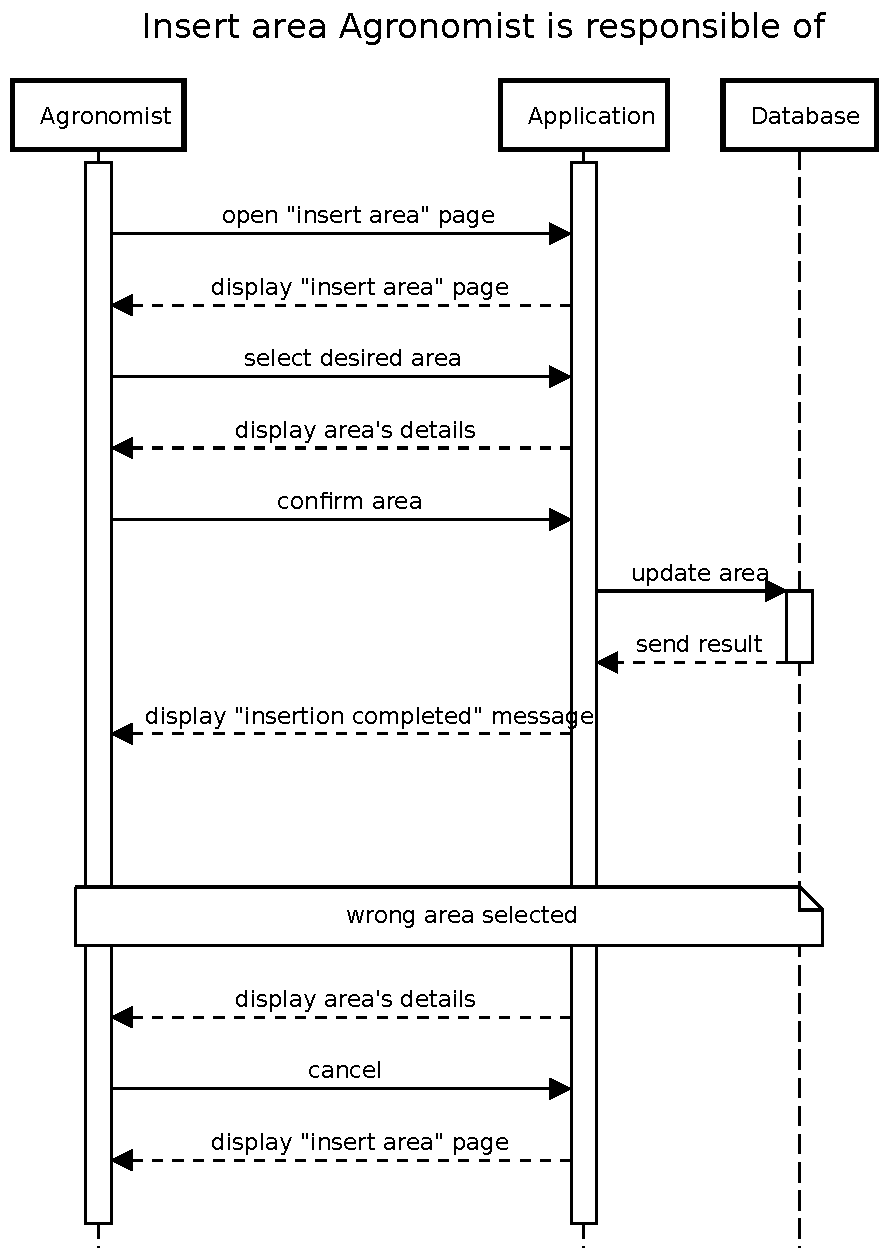
\includegraphics[scale=0.75]{Images/Sequence diagrams/Agronomist - Insert area.pdf}

    \caption{Add an area for an agronomist - sequence diagram}
    \label{fig:fig:seq_diag_insert_area}

    
\end{figure}


% USE CASE 2: REMOVING AN AREA UNDER THE AGRONOMIST'S RESPONSIBILITY
\begin{table}[H]
    \centering
    \begin{tabular}[c]{|l|p{0.75\textwidth}|}
        \hline % ---------------------------------------------------------------------
    	\textsc{id}                 &   A.2\\
    	\hline % ---------------------------------------------------------------------
    	\textsc{Name}               &   Remove an area under the agronomist's responsibility\\
    	\hline % ---------------------------------------------------------------------
    	\textsc{Actor}             &   Agronomist\\
    	\hline % ---------------------------------------------------------------------
    	\textsc{Entry conditions}   &  
    	\begin{itemize}
                                    	    \item Agronomist has logged in
                                    	    \item Agronomist is responsible for at least one area
                                        \end{itemize}\\
    	\hline % ---------------------------------------------------------------------
    	\textsc{Events flow}         &   %\footnotesize
            	                        \begin{itemize}
                                    	    \item Agronomist goes to the "Area management" section
                                    	    \item The system extracts the data from the database and displays the list of areas under the agronomist's responsibility
                                    	    \item Agronomist presses the button “Remove this area” next to the desired area
                                    		\item The system displays a popup asking for confirmation
                                    		\item Agronomist clicks on “Confirm”
                                    		\item The system updates the database and shows a message of removal completed
                                        \end{itemize}\\
        \hline % ---------------------------------------------------------------------
        \textsc{Exit condition}    &  The system displays the "Area management" section\\
    	\hline % ---------------------------------------------------------------------
    	\textsc{Output}             &  \begin{itemize}
    	    \item The system has removed the agronomist in the database as responsible for that area
    	\end{itemize}\\
    	\hline % ---------------------------------------------------------------------
    	\textsc{Exception}         &  Agronomist wrongly clicks “Remove this area”. The system displays a popup notifying that he will be removed as responsible for that area and the agronomist clicks on “Cancel” button\\
    	\hline % ---------------------------------------------------------------------
        
    \end{tabular}
    \caption{\label{tab:responsible_area_insertion}Remove an area for an agronomist}
\end{table}

% USE CASE TABLE 2: ACCESS THE "REQUEST FOR HELP" SECTION

\begin{table}[H]
    \centering
    \begin{tabular}[c]{|l|p{0.75\textwidth}|}
        \hline % ---------------------------------------------------------------------
    	\textsc{id}                 &   A.3\\
    	\hline % ---------------------------------------------------------------------
    	\textsc{Name}               &   Visualize and answer to requests for help\\
    	\hline % ---------------------------------------------------------------------
    	\textsc{Actor}             &   Agronomist\\
    	\hline % ---------------------------------------------------------------------
    	\textsc{Entry condition}   &   Agronomist has logged in\\
    	\hline % ---------------------------------------------------------------------
    	\textsc{Events flow}         &   %\footnotesize
            	                        \begin{itemize}
                                    	    \item Agronomist goes to the “Requests for help” section
                                    		\item The system extracts the data from the database and displays a search bar and the list of conversations (sorted by recent activity), marking the ones which contains new messages
                                    		\item Agronomist selects a conversation
                                    		\item The system displays all the messages contained in that conversation and a text box
                                    		\item Agronomist writes in the text box an answer to the request and clicks “Send”
                                    		\item The system adds the message to the database
                                        \end{itemize}\\
        \hline % ---------------------------------------------------------------------
        \textsc{Exit condition}    &  The system remains in the same page, refreshing its content\\
    	\hline % ---------------------------------------------------------------------
    	\textsc{Output}             &  \begin{itemize}
    	    \item The system adds the message to the database
    	    \item The system notifies the participants of that conversation about the new message
    	\end{itemize}\\
    	\hline % ---------------------------------------------------------------------
    	\textsc{Exception}         &  The system cannot connect to the database/server. The system displays an error message.\\
    	\hline % ---------------------------------------------------------------------
        
    \end{tabular}
    \caption{\label{tab:help_request_section_access}Visualize and answer to requests for help}
\end{table}

\begin{figure}[H]
    \centering
    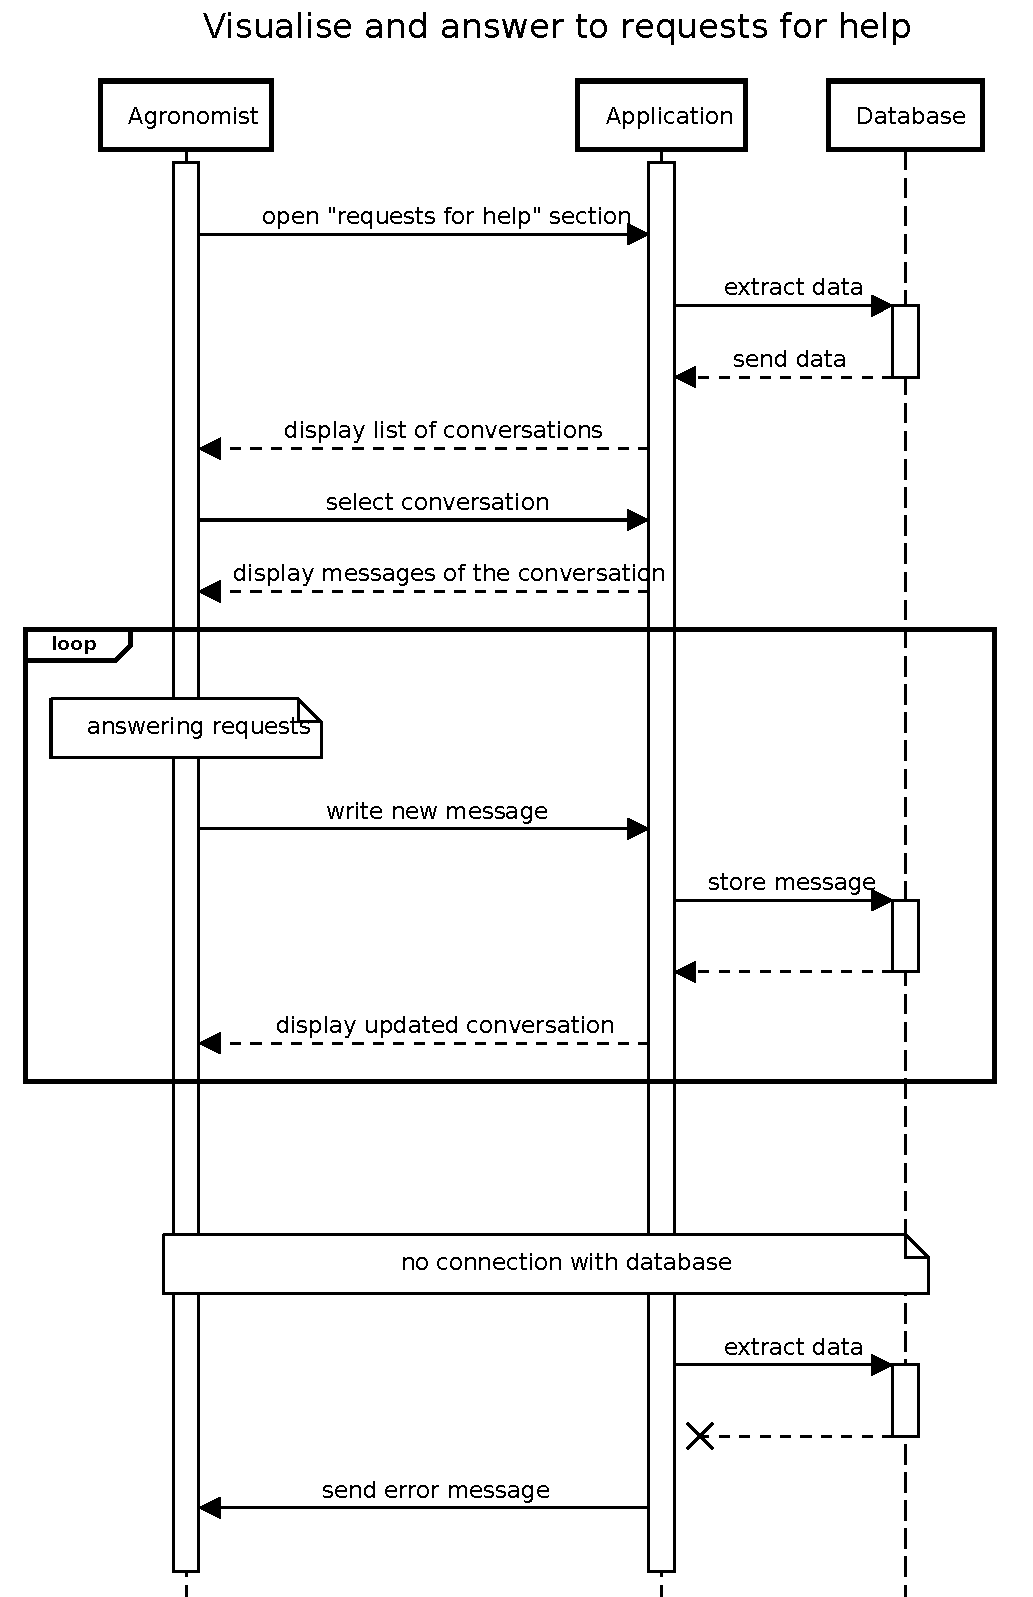
\includegraphics[scale=0.75]{Images/Sequence diagrams/Agronomist - visualise and answer requests for help.pdf}

    \caption{Visualize and answer to requests for help - sequence diagram}
    \label{fig:fig:seq_diag_answer_request}
\end{figure}

% USE CASE TABLE 3: VISUALIZE DATA OF THE AREA

\begin{table}[H]
    \centering
    \begin{tabular}[c]{|l|p{0.75\textwidth}|}
        \hline % ---------------------------------------------------------------------
    	\textsc{id}                 &   A.4\\
    	\hline % ---------------------------------------------------------------------
    	\textsc{Name}               &   Visualize data of an area\\
    	\hline % ---------------------------------------------------------------------
    	\textsc{Actor}             &   Agronomist\\
    	\hline % ---------------------------------------------------------------------
    	\textsc{Entry condition}   &   Agronomist has logged in\\
    	\hline % ---------------------------------------------------------------------
    	\textsc{Events flow}         &   %\footnotesize
            	                        \begin{itemize}

                                    	    \item Agronomist goes to the “Information about areas” section
                                    	    \item The system extract the data from the database and displays the list of areas under the agronomist's responsibility
                                    	    \item Agronomist selects an area
                                    		\item The system displays a page with three main options: “Weather forecasts”, “Farmers’ performing situation” and "Problems encountered"
                                    		\item Agronomist selects  the “Weather forecasts” section
                                    		\item The system extracts the data from the database and shows all the information concerning the weather forecasts in that area
                                    		\item Agronomist selects the “Farmers’ performing situation” section
                                    		\item The system extracts the data from the database and displays the list of all the farmers in the area, grouping them in “Best performing”, “Normal performing” and “Under-performing”
                                    		\item Agronomist selects a farmer
                                    		\item The system displays detailed information about that farmer (overall situation, planned visits, past visits, problems encountered)
                                    		\item Agronomist selects the "Problems encountered" section
                                    		\item The system displays the list of problems inserted by the farmers belonging to the Agronomist's area
                                        \end{itemize}\\
        \hline % ---------------------------------------------------------------------
        \textsc{Exit condition}    &  The system returns to the main page\\
    	\hline % ---------------------------------------------------------------------
    	\textsc{Exceptions}         &  The system cannot connect to the database/server. The system displays an error message.
    	\\
    	\hline % ---------------------------------------------------------------------
        
    \end{tabular}
    \caption{\label{tab:Area_information_access}Visualize data of an area}
\end{table}

\begin{figure}[H]
    \centering
    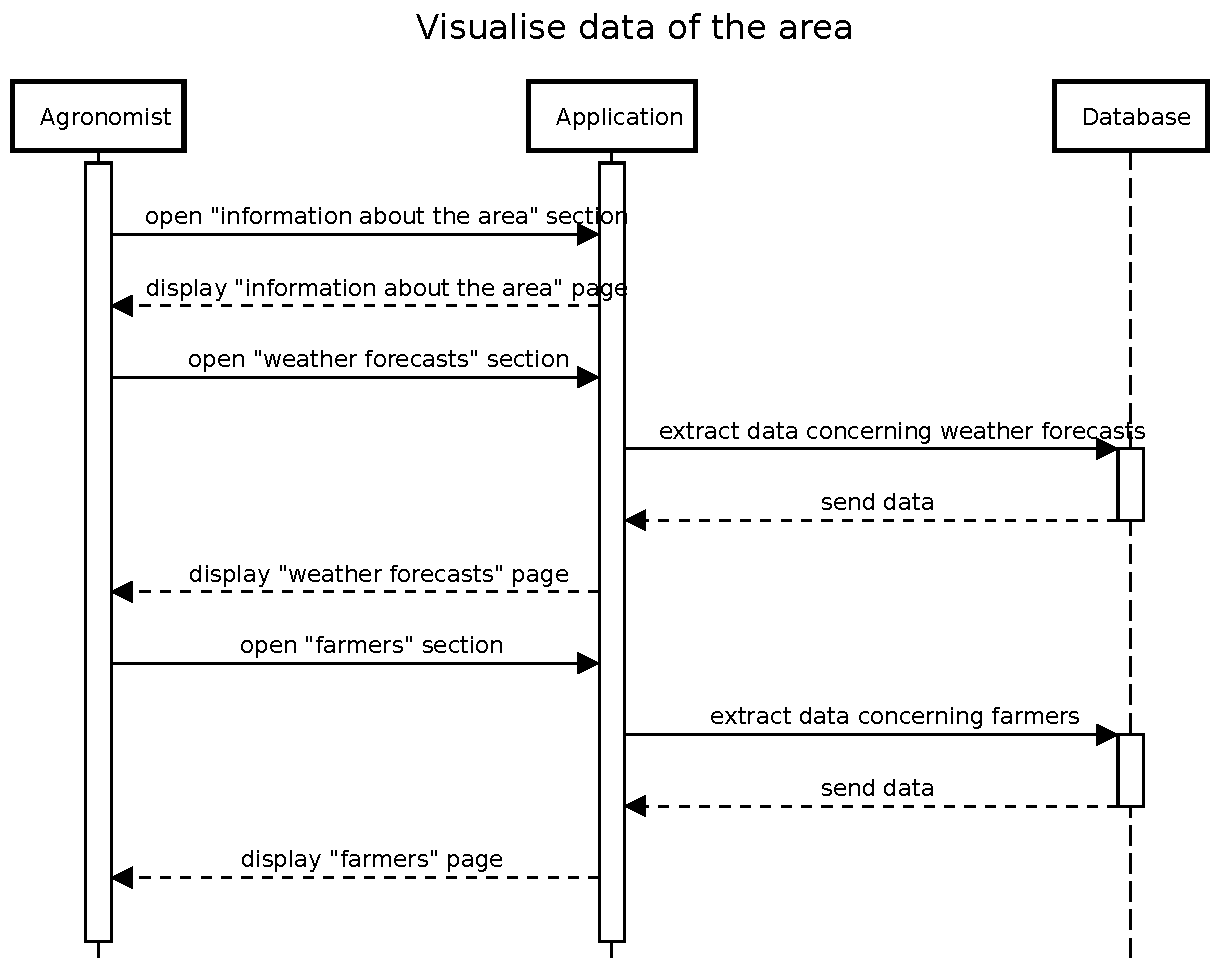
\includegraphics[scale=0.65]{Images/Sequence diagrams/Agronomist - visualise data of the area.pdf}

    \caption{Visualize data of an area - sequence diagram}
    \label{fig:fig:seq_diag_visualize_area}
\end{figure}

% USE CASE TABLE 4: ACCESS THE "DAILY PLAN" SECTION


\begin{table}[H]
    \centering
    \begin{tabular}[c]{|l|p{0.75\textwidth}|}
        \hline % ---------------------------------------------------------------------
    	\textsc{id}                 &   A.5\\
    	\hline % ---------------------------------------------------------------------
    	\textsc{Name}               &   Visualize and update a daily plan\\
    	\hline % ---------------------------------------------------------------------
    	\textsc{Actors}             &   Agronomist\\
    	\hline % ---------------------------------------------------------------------
    	\textsc{Entry conditions}   &   \begin{itemize}
                                    	    \item Agronomist has logged in
                                    	    \item At least one daily plan is present
                                        \end{itemize}\\
    	\hline % ---------------------------------------------------------------------
    	\textsc{Events flow}         &   %\footnotesize
            	                        \begin{itemize}
                                    	    \item Agronomist goes to the “Daily Plan” section, which is divided in “Visualize/Update” and “Confirm/Specify deviation from”. Agronomist selects the “Visualise/Update” section
                                    		\item The system extracts the data from the database and displays the list of daily plans for that agronomist
                                    		\item Agronomist selects a daily plan
                                    		\item The system displays all the information about that daily plan (day-month-year, farmers to be visited)
                                    		\item Agronomist clicks on the “Update” button
                                    		\item The system displays the list of farmers contained in the selected daily plan
                                    		\item Agronomist clicks on the “Remove” button near the farmer he wants to remove
                                            \item The systems displays the updated list of farmers
                                            \item Agronomist clicks on the “Add farmer” button
                                            \item The system displays the list of all the farmers for which the agronomist is responsible of and that are not already in the selected daily plan. In addition, for each farmer it is shown the list of problems encountered and the list of past and future visits (planned also by other agronomists) in a sort of compact calendar
                                            \item Agronomist selects a subset of farmers and clicks on “Add”
                                            \item The system displays the updated list of farmers
                                            \item Agronomist checks the info and clicks on “Confirm changes”

                                        \end{itemize}\\
        \hline % ---------------------------------------------------------------------
        \textsc{Exit condition}    &  The system shows a popup to notify the agronomist of the success of the operation
        \\
    	\hline % ---------------------------------------------------------------------
    	\textsc{Output}             &  \begin{itemize}
    	    \item The updated daily plan is stored in the database
    	\end{itemize}\\
    	\hline % ---------------------------------------------------------------------
    	\textsc{Exceptions}         &  \begin{itemize}
    	    \item The selected daily plan has already been confirmed and cannot be updated anymore. The system shows an error message.
    	    \item The selected daily plan is referring to the current day and cannot be updated anymore. The system shows an error message.
    	    \item Agronomist has made the wrong modifications to the daily plan. Instead of clicking “Confirm changes”, he/it clicks on “Discard changes”. The system displays the original daily plan and doesn’t store the new one in the database.    	\end{itemize}\\
    	
    	\hline % ---------------------------------------------------------------------
        
    \end{tabular}
    \caption{\label{tab:daily_plan_section_access}Visualize and update a daily plan}
\end{table}

\begin{figure}[H]
    \centering
    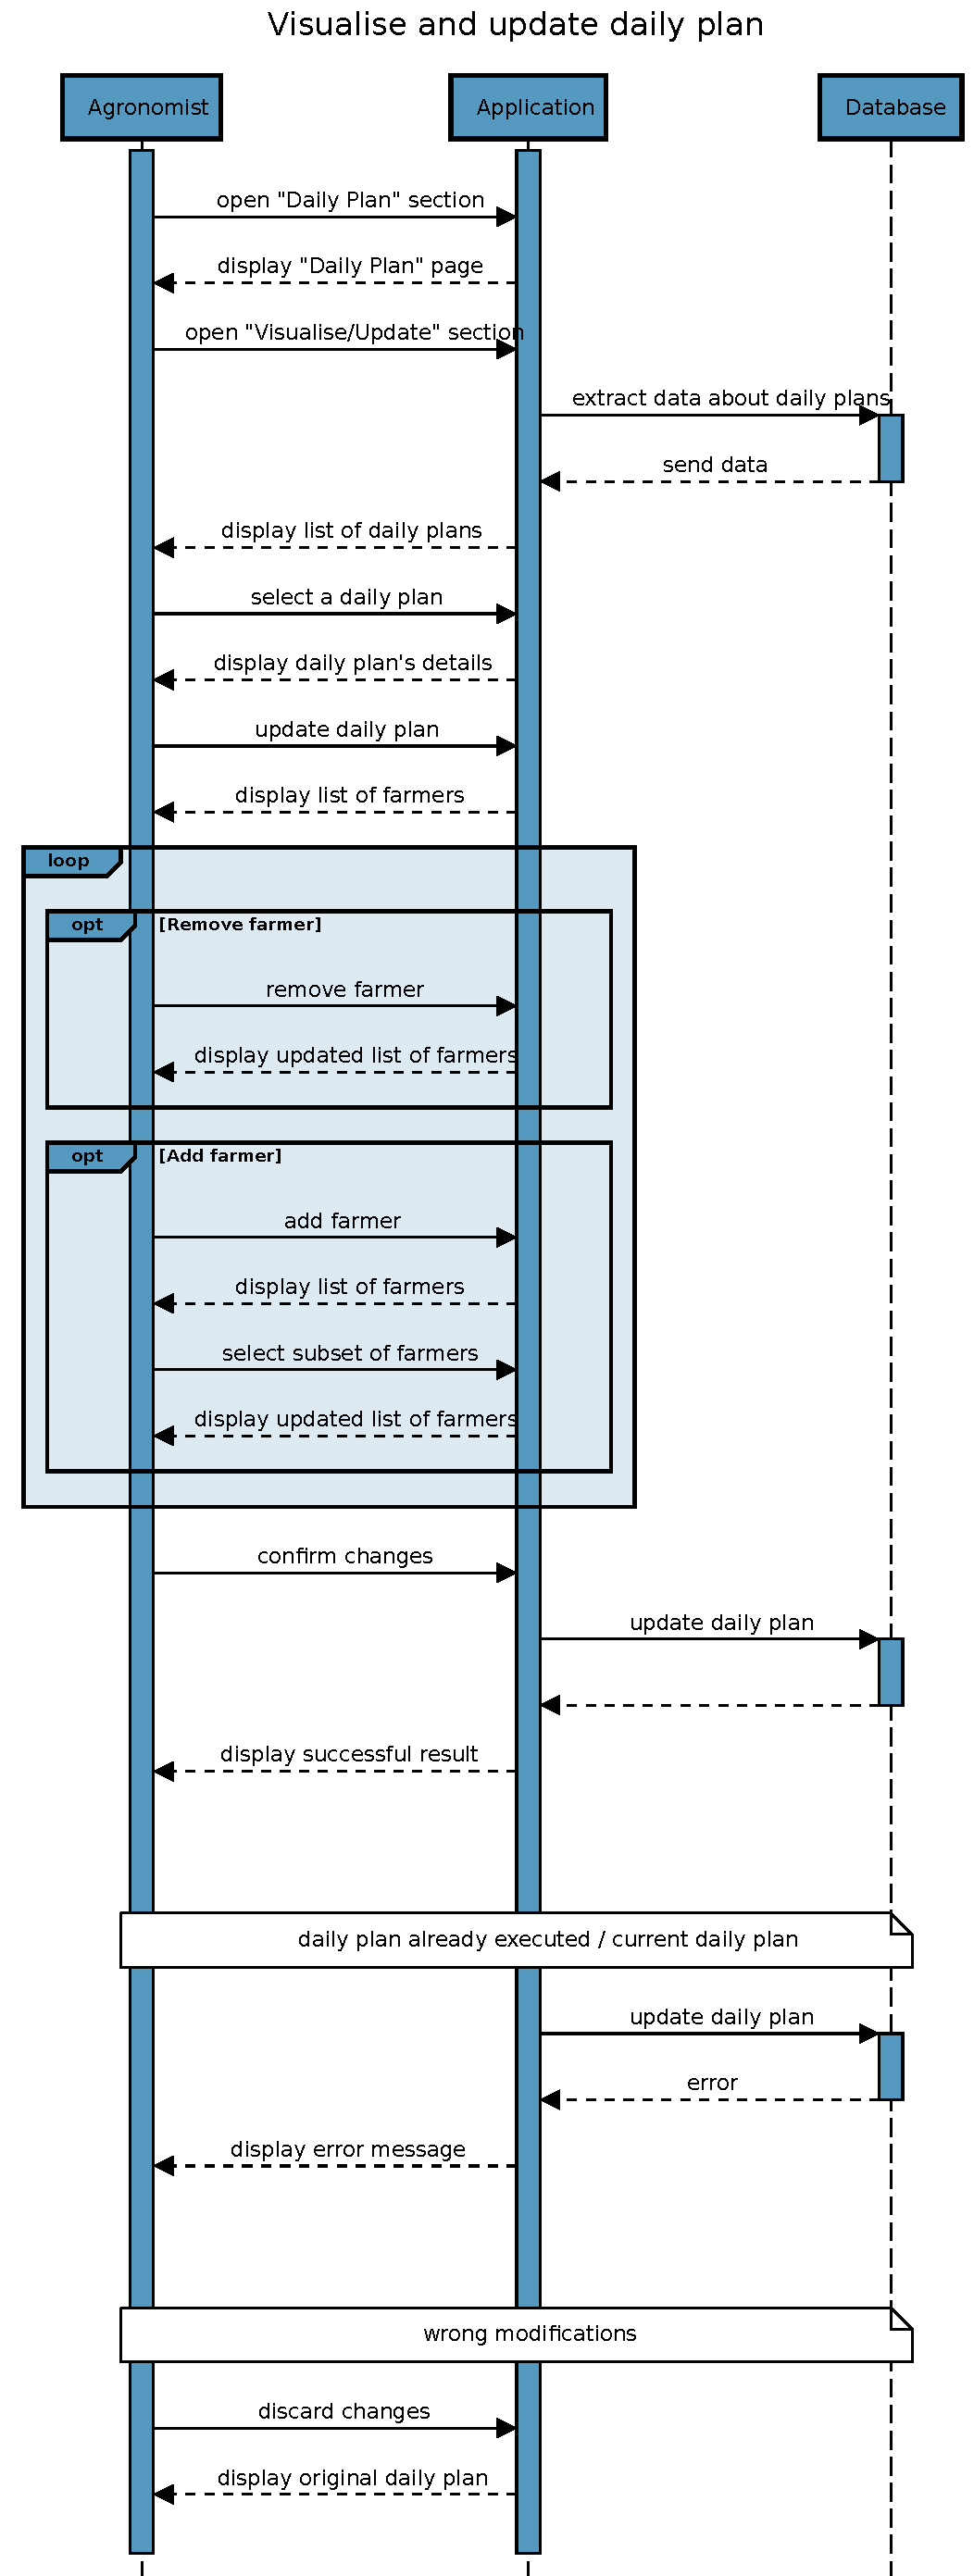
\includegraphics[scale=0.45]{Images/Sequence diagrams/Agronomist - visualise and update daily plan.pdf}

    \caption{Visualize and update a daily plan - sequence diagram}
    \label{fig:fig:seq_diag_update_daily_plan}
\end{figure}

% USE CASE TABLE 5: CONFIRM DEVIATIONS FROM DAILY PLAN


\begin{table}[H]
    \centering
    \begin{tabular}[c]{|l|p{0.75\textwidth}|}
        \hline % ---------------------------------------------------------------------
    	\textsc{id}                 &   A.6\\
    	\hline % ---------------------------------------------------------------------
    	\textsc{Name}               &   Confirm execution of daily plan\\
    	\hline % ---------------------------------------------------------------------
    	\textsc{Actor}             &   Agronomist\\
    	\hline % ---------------------------------------------------------------------
    	\textsc{Entry conditions}   &   \begin{itemize}
                                    	    \item Agronomist has logged in
                                    	    \item Agronomist has at least one daily plan
                                        \end{itemize}\\
    	\hline % ---------------------------------------------------------------------
    	\textsc{Events flow}         &   %\footnotesize
            	                        \begin{itemize}
                                    	    \item Agronomist goes to the “Daily Plan” section, which is divided in “Visualize/Update” and “Confirm/Specify deviation from”. Agronomist selects the “Confirm/Specify deviation from” section.
                                    		\item The system extracts the data from the database, displays the daily plan for the current day and enables the agronomist to select the subset of farmers which has not been visited that day
                                            \item Agronomist checks the info, selects the subset of farmers and clicks on “Continue”
                                            \item The system displays a compact summary of the info and asks for confirmation
                                            \item Agronomist checks the info and clicks on “Confirm”

                                        \end{itemize}\\
        \hline % ---------------------------------------------------------------------
        \textsc{Exit condition}    &  The system shows a popup to notify the agronomist of the success of the operation
        \\
    	\hline % ---------------------------------------------------------------------
    	\textsc{Output}             &  \begin{itemize}
    	    \item The system stores the completed daily plan in the database, 
            \item The system increments by one the number of visits received by the farmers that actually have been visited
            \item The system rearranges the non-visited farmers in future daily plans

    	\end{itemize}\\
    	\hline % ---------------------------------------------------------------------
    	\textsc{Exception}         &  Agronomist has selected the wrong subset of farmers. Given the compact summary, it clicks on “Cancel”. The system displays again the daily plan and enables the agronomist to choose another subset of farmers.\\
    	
    	\hline % ---------------------------------------------------------------------
        
    \end{tabular}
    \caption{\label{tab:confirm_deviations_section}Confirm execution of daily plan}
\end{table}

\begin{figure}[H]
    \centering
    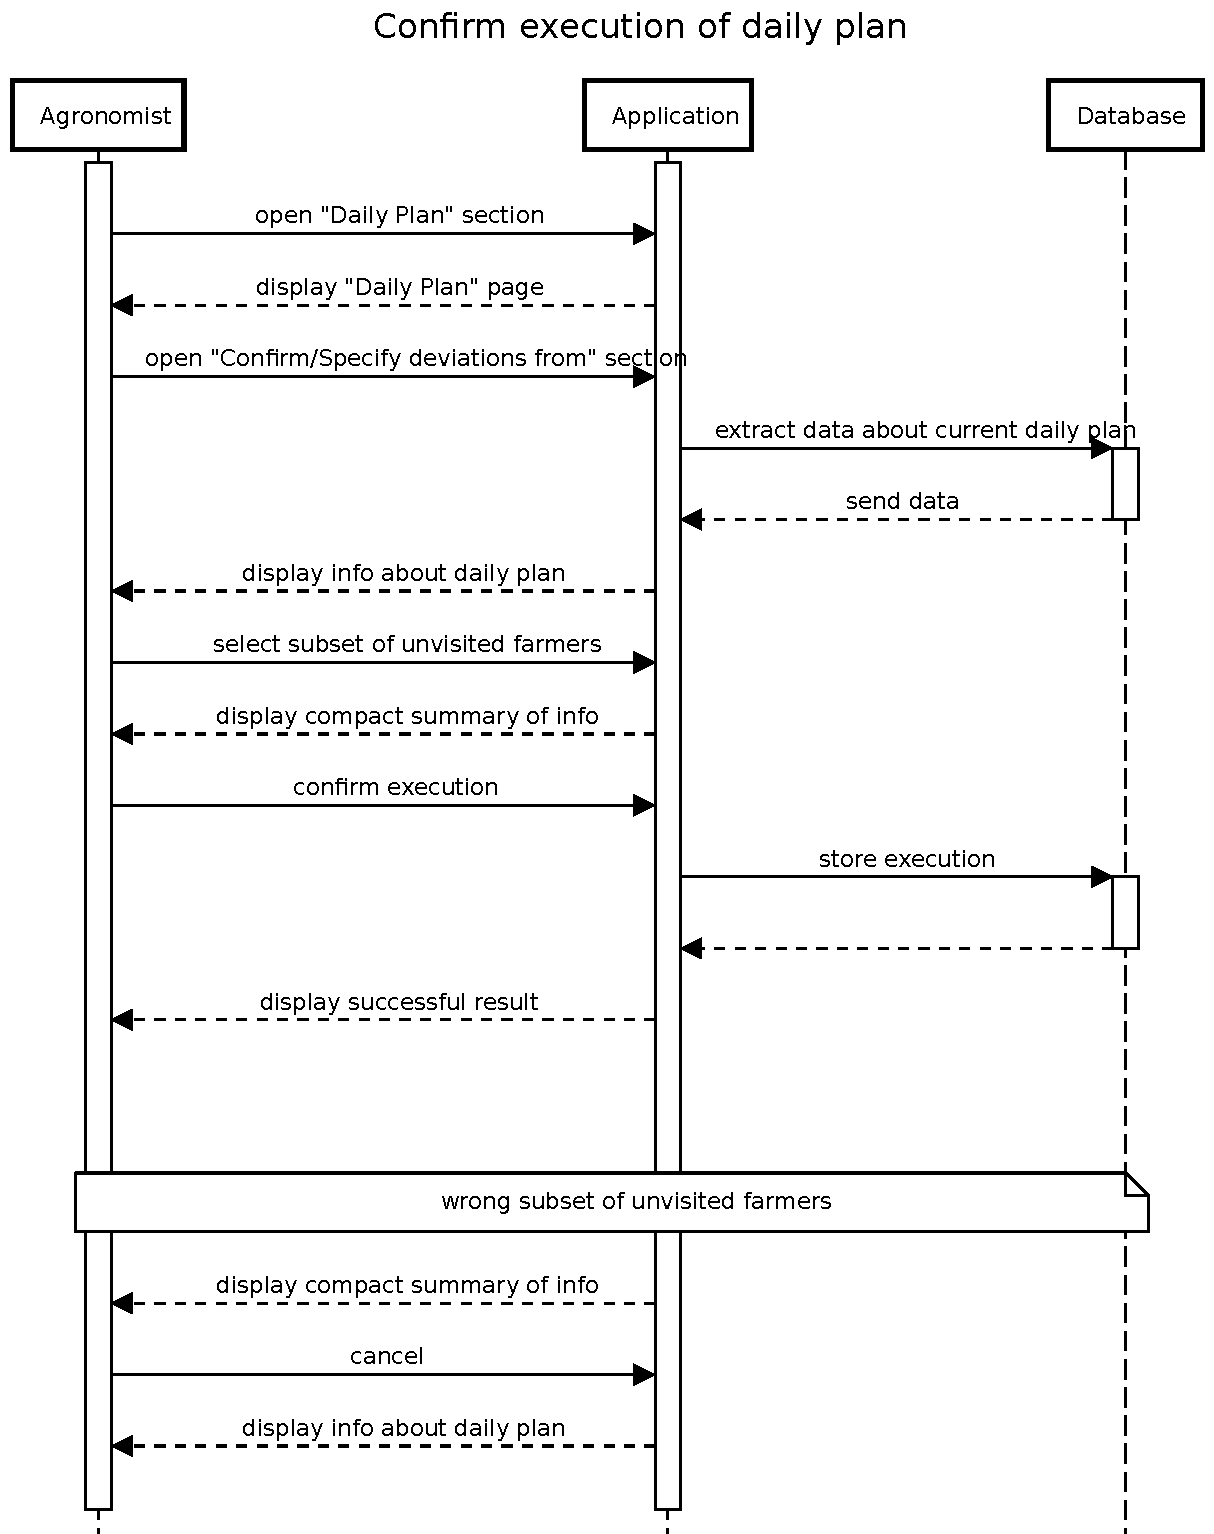
\includegraphics[scale=0.75]{Images/Sequence diagrams/Agronomist - confirm execution of daily plan.pdf}

    \caption{Confirm execution of daily plan - sequence diagram}
    \label{fig:fig:seq_diag_confirm_daily_plan}
\end{figure}